\chapter*{Программа}

Во время работы были написаны следующие программы:
\begin{enumerate}
    \item mesher - программа для генерации рассчётной сетки для системы
    \item solver - программа для рассчёта деформаций и разрыва тканного композита
\end{enumerate}
Далее подробно рассмотрим каждую программу.

\section*{Mesher}
Mesher - программа для генерации рассчётной сетки для системы.
Написана на языке Python.

На верхнем уровне состоит из следующих частей:
\begin{enumerate}
    \item config - модуль для чтения конфигурационных файлов
    \item mesher - основная часть, которая занимается генерацией in-memory сетки
    \item writer - вспомогательный модуль для записи сетки на диск
\end{enumerate}

\subsection*{Config}
Модуль config предназначен для чтения конфигурационных файлов.

Формат конфигурационных файлов основан на YAML, что позволяет в будущем расширить формат практически без
изменения исходного кода.

Конфиг представляет собой список задач (tasks) и директорию, для записи результатов (out\_dir).
Каждый task имеет вид
\begin{minted}{yaml}
name: simple # название таска, результат будет иметь вид: name.vtu
  resolution: 100 # Разрешение нитей, точек/см
  diameter: 0.5 # толщина нити, см
  width: 20 # Ширина куска = длина ниток утка
  weft_density: 1 # Плотность ниток утка, нитей / см
  length: 50 # Длина куска = длина ниток основы
  warp_density: 0.5 # Плотность ниток основы, нитей / см
\end{minted}

Он описывает один слой из переплетённых нитей утка и основы.

\begin{figure}[H]
    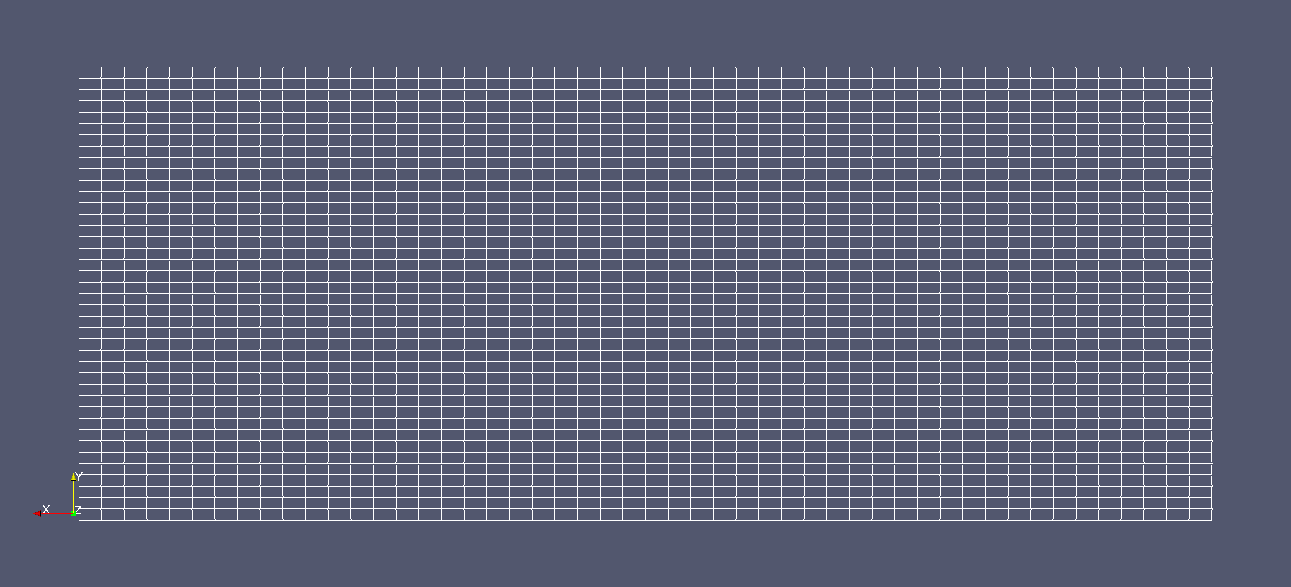
\includegraphics[width=0.8\textwidth]{img/scheme.png}
    \centering
\end{figure}

В дальнейшем планируется расширить конфиг, с целью добавить поддержку описания многослойных конструкций
и переменной плотности намотки.

\subsection*{Mesher}
Mesher - основной модуль в программе.
Генерирует сетку для слоя ткани.

Основной алгоритм:

Разделяем ткань на два вида нитей - основа и уток

Для основы: генерируем mesh для одной прямой нити.
Повторяем
\[
    N = length * warp\_density
\]
параллельным переносом на
\[
    d = \frac{1}{warp\_density}
\]


Для утка: генерируем mesh для одной оплетающейся нити
\begin{minted}{python}
    def create_weft(width: float, length: float, density: int, diameter: float,
                    warp_density: float,
                    resolution: float) -> Layer:
        def fn(t: float) -> Point:
            r = diameter / 2
            d = 1 / warp_density

            if t < r:
                return Point(
                    x=0,
                    y=t,
                    z=math.sqrt(r ** 2 - t ** 2),
                )
            elif t < d - r:
                return Point(
                    x=0,
                    y=t,
                    z=0,
                )
            elif t < d + r:
                return Point(
                    x=0,
                    y=t,
                    z=-math.sqrt(r ** 2 - (t - d) ** 2),
                )
            elif t < 2 * d - r:
                return Point(
                    x=0,
                    y=t,
                    z=0,
                )
            elif t < 2 * d:
                return Point(
                    x=0,
                    y=t,
                    z=math.sqrt(r ** 2 - (t - 2 * d) ** 2),
                )
            else:
                n_periods = int(t / (2 * d))
                p = fn(t - n_periods * 2 * d)

                return p + Point(x=0, y=2 * d * n_periods, z=0)

        fibers_step = 1 / density
        n_fibers = int(density * width)
        points_step = 1 / resolution
        n_points = int(length / points_step)
        root_fiber = create_fiber(fn, points_step, n_points)

        fibers = [root_fiber]
        dp = Point(x=fibers_step, y=0, z=0)
        for i in range(n_fibers - 1):
        fibers.append(fibers[-1].shift(dp=dp))

        return Layer(fibers=fibers)
\end{minted}

Получим нить вида:
\begin{figure}[H]
    \centering
    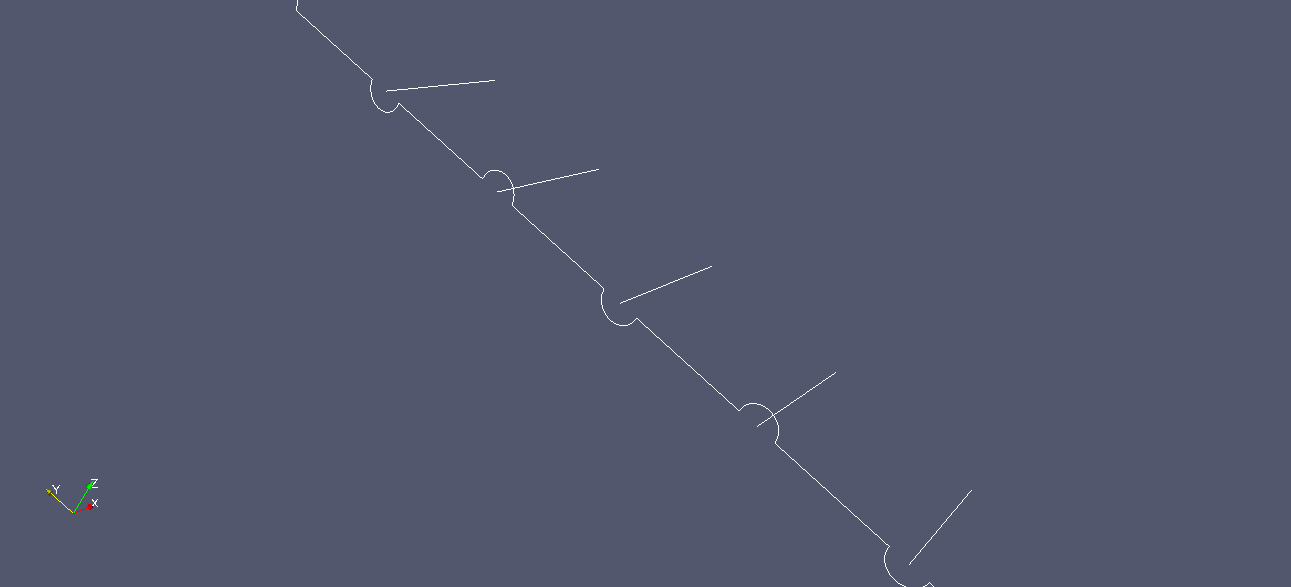
\includegraphics[width=0.8\textwidth]{img/weft_fiber.png}
\end{figure}

Для простоты на данном этапе считаем, что нить утка оплетается по чередующимся полуокружностям.

И как и в пункте про основу повторяем
\[
    N = width * weft\_density
\]
параллельным переносом на
\[
    d = \frac{1}{weft\_density}
\]

\subsection*{Writer}
Writer - модуль, отвечающий за запись сетки в формат .vtu (VTK Unstructured grid).

